\documentclass{iopart}
\usepackage{arydshln}
\usepackage{multirow}
\usepackage{amsopn}
\usepackage{iopams}
\usepackage{graphicx}
\usepackage{bib/aas_macros}
\usepackage[colorlinks]{hyperref}
\input{ligo-acronyms/acronyms}

% From http://www.f.kth.se/~ante/latex.php
\setlength{\marginparwidth}{1.2in}
\let\oldmarginpar\marginpar
\renewcommand\marginpar[1]{\-\oldmarginpar[\raggedleft\footnotesize #1]%
{\raggedright\footnotesize #1}}

\DeclareMathOperator{\cov}{cov}
\DeclareMathOperator{\std}{std}
\DeclareMathOperator*{\argmin}{\arg\!\min}
\DeclareMathOperator*{\argmax}{\arg\!\max}

\begin{document}

\title[Rapid-response Bayesian sky localization]{Rapid-response Bayesian sky localization for electromagnetic follow-up of gravitational-wave candidates}
\author{Leo Singer and Larry R. Price}
\address{\acs{LIGO} Laboratory, California Institute of Technology, Pasadena, CA 91125, USA}
\ead{\mailto{leo.singer@ligo.org}, \mailto{larryp@caltech.edu}}

\begin{abstract}
Timely \acl{EM} follow\nobreakdashes-up of \acl{CBC} events detected by \acl{aLIGO} requires rapidly inferring the sky location from the \ac{GW} observations. Calculation of the posterior distribution of the sky location and intrinsic source parameters given the \ac{GW} strain takes hours with state\nobreakdashes-of\nobreakdashes-the\nobreakdashes-art \ac{MCMC} parameter estimation codes. By taking as the measurement not the \ac{GW} strain itself but the amplitude and \acl{TOA} of the putative signal at each detector, and by fixing the intrinsic source parameters, we have constructed a non-\ac{MCMC}, fully deterministic Bayesian parameter estimation algorithm that takes just seconds to produce sky maps of posterior probability.%
\marginpar{Wrong emphasis? I like Larry's idea of having this paper discuss several different tiers of sky localization with increasing accuracy and latency.}
\end{abstract}

\section{Outline}

\begin{enumerate}
\item Introduction {
	\begin{enumerate}
	\item Background: \acp{GRB}, \acp{CBC}, \acs{LIGO}
	\item Time scales of \acp{GRB}, \acp{CBC}
	\item Current sky localization algorithms and response times
	\end{enumerate}
}
\item Preliminaries {
	\begin{enumerate}
	\item Fisher information, \ac{CRLB}
	\item Matched\nobreakdashes-filter estimator
	\end{enumerate}
}
\item Algorithm {
	\begin{enumerate}
	\item Assumptions
	\item Signal model
	\item Likelihood function
	\item Priors and marginalization
	\item Procedure
	\end{enumerate}
}
\item Results {
	\begin{enumerate}
	\item Injection population
	\item Cumulative fraction vs. confidence level plots
	\item Sky localization accuracy as a function of distance or \ac{SNR}
	\item Speed
	\end{enumerate}
}
\item Discussion {
	\begin{enumerate}
	\item Potential further refinements
	\item What astrophysical targets were accessible before
	\item What new targets are available with the response time of seconds
	\item Lay out timeline of follow\nobreakdashes-up campaign, including different tiers of inference and different types of telescopes
	\end{enumerate}
}
\item Appendices {
	\begin{enumerate}
	\item Code listing?
	\item Any proofs that are needed in the body but would interrupt the text?
	\end{enumerate}
}
\end{enumerate}


\section{Introduction}

Ground-based \ac{GW} interferometers are entering the advanced detector era, positioning themselves to make profound discoveries about the universe. The \ac{aLIGO} and Vigo detectors will be part of a worldwide network that also includes KAGRA and hopefully LIGO-India. Coalescing neutron star binaries are among the most likely sources, with event rates of $~ 50/\mathrm{yr}$~\cite{rates}.%
%
\marginpar{Check that number.}%
%
In addition to being an efficient source of \acp{GW}, the \ac{NS} may be tidally shredded before merging, providing fuel for an electromagnetic counterpart. The short-lived accretion flow may power a collimated relativistic jet, resulting in a short \ac{GRB} and an X-ray afterglow if it is aligned with the line of sight. An optical afterglow may follow minutes to hours later as the jet plows into the interstellar medium. As surrounding neutron-rich ejecta decay radioactively, an optical `kilonova' may be visible after $\sim$1 day \cite{metzger:2010}. Finally, as the ejecta plow into the interstellar medium, a faint radio afterglow could occur on a timescale of weeks to years \cite{Nakar:2011cw}.

There is therefore a strong case for performing electromagnetic followups of these sources of \acp{GW}. Indeed, the final science run of the intitial LIGO and Virgo instruments saw the first joint search for \acp{GW} from compact binaries and their electromagnetic counterparts \cite{abadie2012first}.  As we prepare for the next generation of these searches there is a need for determining the location of the source as precisely as possible in as little time as possible.

In this paper we present a rapid and accurate method of sky localization that makes use of Bayesian methods. It differs from existing techniques is several important ways.  In the first place, we fix the intrinsic parameters to their \ac{ML} estimates, as provided by the detection pipeline.  This reduces the dimensionality of the parameter space we need to sample. In addition, the technique takes as its input the \ac{ML} estimates of the extrinsic parameters, instead of the $h(t)$ time series. This makes the likelihood itself much faster to evaluate. Finally, instead of of using \ac{MCMC} or some similar method for statistical sampling, we make use of a deterministic quadrature scheme. We call this technique \ac{BAYESTAR}%
%
\footnote{A pun on the Cylon battleships in the American television series Battlestar Galactica. The defining characteristic of the Cylons is that they repeatedly defeat humanity by using their superhuman information\nobreakdashes-gathering ability to coordinate overwhelming forces. The name also suggests that, like the Cylons, \acp{GW} detectors may some day rise against us humans.}%
%
\footnote{We do not like to mention the final `T' in the acronym, because then it would be called BAYES\nobreakdashes-TART, which would sound ridiculous.}%
. It is unique in that in bridges the detection and parameter estimation of \ac{GW} signals, two tasks that have until now involved very different numerical methods and time scales. We expect that \ac{BAYESTAR} will take on a key role in observing \ac{CBC} events in both \ac{GW} and optical channels during the Advanced \ac{LIGO} era.

\section{Theory of \ac{GW} detection and parameter estimation}

A laser interferometer senses \acp{GW} by transducing differential changes in arm length to a digitized photocurrent time series. In the angular frequency domain, a single detector's observation $X_i(\omega)$ is
%
\begin{equation}\label{eq:signal-model}
	x_i (\omega) = h_i (\omega; \boldsymbol\theta) + n_i (\omega),
\end{equation}
%
where $h_i (\omega; \boldsymbol\theta)$ is the \ac{GW} signal receied by detector $i$, given a parameter vector $\boldsymbol\theta$ that describes the \ac{GW} source, and $n_i (\omega)$ is that detector's \ac{WSS} Gaussian noise with \ac{PSD} $S_i(\omega)$. We shall denote the combined observation from a network of detectors as $\mathbf x (\omega) \equiv \{x_i (\omega)\}_i$.

The likelihood, or the probability of obtaining the observation $\mathbf x$ conditioned on the value of $\boldsymbol\theta$, is Gaussian, with the log\nobreakdashes-likelihood proportional to:
%
\begin{equation}\label{eq:gaussian-likelihood}
	\mathcal{L}(\mathbf x; \boldsymbol\theta) = \prod_i p(x_i | \boldsymbol\theta)
		\propto \exp \left[
		- \frac{1}{2} \sum_i \int_0^\infty \frac{\left|x_i (\omega)
			- h_i(\omega; \boldsymbol\theta) \right|^2}{S_i(\omega)} \, \mathrm{d}\omega
	\right].
\end{equation}

A \ac{CBC} source is specified by a vector of extrinsic parameters describing its position and orientation and intrinsic parameters describing the physical properties of the binary components:
%
\begin{equation}
    \boldsymbol\theta = \begin{array}{l@{}l}
            \left[
            \begin{array}{c}
                \alpha \\
                \delta \\
                D_\mathrm{L} \\
                t_\oplus \\
                u \\
                \psi \\
                \phi_c \\
                \hdashline[1pt/1pt]
                m_1 \\
                m_2 \\
                \mathbf S_1 \\
                \mathbf S_2
            \end{array}
            \right] &
            \begin{array}{l}
                \left.
                \begin{array}{p{4cm}}
                    right ascension \\
                    declination \\
                    luminosity distance \\
                    arrival time at geocenter \\
                    $\cos(\textrm{inclination angle})$ \\
                    polarization angle \\
                    coalescence phase \\
                    \hdashline[1pt/1pt]
                \end{array}
                \quad \right\} \textnormal{extrinsic parameters}, \boldsymbol\theta_\mathrm{ex} \\
                \left.
                \begin{array}{p{4cm}}
                    first component's mass \\
                    second component's mass \\
                    first component's spin \\
                    second component's spin
                \end{array}
                \quad \right\} \textnormal{intrinsic parameters}, \boldsymbol\theta_\mathrm{in}
            \end{array}
        \end{array}
\end{equation}
%
Binary eccentricity is omitted as an intrinisc parameter because tidal interaction of the progenitor stars~\cite{0004-637X-572-1-407} and later \ac{GW} emission~\cite{PhysRev.136.B1224} circularize the orbit long before the inspiral enters \ac{LIGO}'s frequency range of $\sim$10\nobreakdashes--1000~kHz. Tidal deformabilities of the \acp{NS} are omitted because the effect of tides on the inspiral would only be detectable by an Einstein Telescope-class \ac{GW} observatory~\cite{PhysRevD.81.123016}. Furthermore, in \ac{GW} detection efforts, especially those focused on \ac{NSNS} systems, the component spins $\mathbf{S}_1$ and $\mathbf{S}_2$ are often assumed to be aligned with the system's total angular momentum and condensed to a single scalar parameter $\chi$, or even neglected entirely, $\mathbf{S}_1 = \mathbf{S}_2 = 0$. In this work we will consider only zero spin.

Assuming circular orbits and no spin precession, we can write the \ac{GW} signal in each detector as a linear combination of two basis waveforms $h_0$ and $h_{\pi/2}$. For nonprecessing systems, $h = h_0$ and $h_{\pi/2}$ are approximately ``in quadrature'' in the same sense as the sine and cosine functions, being nearly orthogonal and out of phase by ${\pi/2}$ at all frequencies. In other words, $h_{\pi/2}(\omega) = i h_0(\omega)$ for all $\omega$. This linear combination isolates all dependence on the extrinsic parameters $\boldsymbol\theta_\mathrm{ex}$ into the coefficients and all dependence on the intrinsic parameters $\boldsymbol\theta_\mathrm{in}$ into the basis waveform,
%
\begin{eqnarray}\label{eq:full-signal-model}
	\fl h_i(\omega; \boldsymbol\theta) &=& e^{-i\omega t_\oplus}\frac{D_{1,i}}{D_\mathrm{L}}
	\left(\begin{array}{cc}
		F_{+,i}(\alpha, \delta, t_\oplus) \\
		F_{\times,i}(\alpha, \delta, t_\oplus)
	\end{array}\right)^\intercal
	\left(\begin{array}{cc}
		\cos{2\psi} & -\sin{2\psi} \\
		\sin{2\psi} & \cos{2\psi}
	\end{array}\right)
	\left(\begin{array}{cc}
		\frac{1}{2}\left(1+u^2\right) & 0 \\
		0 & u
	\end{array}\right) \nonumber\\\fl &\cdot&
	\left(\begin{array}{cc}
		\cos{2\phi_c} & -\sin{2\phi_c} \\
		\sin{2\phi_c} & \cos{2\phi_c}
	\end{array}\right)
	\left(\begin{array}{cc}
		1 \\
		i
	\end{array}\right) h(\omega; \boldsymbol\theta_\mathrm{in}).
\end{eqnarray}
%
This linear combination matches the conventions used in \cite{PhysRevD.83.084002}, and is the frequency-domain equivalent of their Equation~(2.8). The quantities $F_{+,i}$ and $F_{\times,i}$ are the dimensionless detector antenna factors, and depend on the orientation of detector $i$ as well as the sky location and sidereal time of the event, and are derived in~\cite{PhysRevD.63.042003}. The quantity $D_{1,i}$ is a fiducial horizon distance for detector $i$,
%
\marginpar{This isn't what we usually call the horizon distance; the horizon distance is where face-on inspirals produce SNR=8.}%
%
\begin{equation}\label{eq:horizon}
D_{1,i} = 1 / \sigma_i, \qquad {\sigma_i}^2 = \int_0^\infty \frac{\left|h(\omega; \mathbf \theta)\right|^2}{S_i(\omega)} \,\mathrm{d}\omega.
\end{equation}

\subsection{Detection, and matched filter bank as a \ac{MLE}}

More succinctly, we can write the signal received by detector $i$ in terms of direct observables, the amplitude $\rho_i$, phase $\gamma_i$, and time delay $\tau_i$ on arrival at detector $i$,
%
\begin{equation}\label{eq:signal-model}
	h_i (\omega; \boldsymbol\theta) = \frac{\rho_i}{\sigma_i} e^{i (\gamma_i - \omega \tau_i)} h(\omega; \boldsymbol\theta_\mathrm{in}).
\end{equation}

The prevailing technique for detection of \acp{GW} from \acp{CBC} is to realize a \ac{MLE} from \Eref{eq:gaussian-likelihood} with the above signal model. This takes the form of a bank of matched filters, or template waveforms that are continually convolved with the incoming data stream. The matched filter or \ac{ML} estimates are given by
%
\begin{eqnarray}
\hat{\boldsymbol\theta}_i, \{\hat\tau_i\}_i &=& \argmax_{\boldsymbol\theta_\mathrm{in}, \{\hat\tau_i\}_i} \sum_i \frac{1}{{\sigma_i}^2} \left| \int_0^\infty \frac{h^*(\omega; \boldsymbol\theta_\mathrm{in}) x_i(\omega) e^{-i \omega \tau_i}}{S_i(\omega)} \,\mathrm{d}\omega \right|^2 \\
\hat\rho_i &=& \frac{1}{\sigma_i} \left| \int_0^\infty \frac{h^*(\omega; \hat{\boldsymbol\theta}_\mathrm{in}) x_i(\omega) e^{-i \omega \hat\tau_i}}{S_i(\omega)} \,\mathrm{d}\omega \right| \\
\hat\gamma_i &=& \arg \int_0^\infty \frac{h^*(\omega; \hat{\boldsymbol\theta}_\mathrm{in}) x_i(\omega) e^{-i \omega \hat\tau_i}}{S_i(\omega)} \,\mathrm{d}\omega,
\end{eqnarray}
%
where the $^*$ denotes a complex conjugate.

\subsection{Bayesian probability and parameter estimation}

In the Bayesian framework, the parameters are inferred from the data by forming the posterior distribution, $p(\boldsymbol\theta|\mathbf x)$, which describes the probability of the parameters given the observations. Bayes' rule relates the likelihood $p(\mathbf x|\boldsymbol\theta)$ to the posterior $p(\boldsymbol\theta|\mathbf x)$,
%
\begin{equation}\label{bayes}
p(\boldsymbol\theta|\mathbf x) = \frac{p(\mathbf x|\boldsymbol\theta) p(\boldsymbol\theta)}{p(\mathbf x)},
\end{equation}
%
introducing the prior distribution $p(\boldsymbol\theta)$ which encapsulates previous information about the paramters (for example, arising from earlier observations or from known physical bounds on the parameters), and the evidence $p(\mathbf x)$ which can be thought of as a normalization factor or as describing the parsimoniousness of the model.

The choice of prior is open to one's astrophysical preconceptions, but during \ac{S6} when \ac{LIGO}'s Bayesian \ac{CBC} parameter estimation pipelines were pioneered, the prior was taken to be isotropic in sky location and binary orientation, and uniform in volume, arrival time, and the component masses~\cite{2013arXiv1304.1775T}. Put briefly, the prior was uniform in all of $(\alpha, \sin\delta, {D_\mathrm{L}}^3, t_\oplus, u, \psi, \phi_c, m_1, m_2)$.

In Bayesian inference, although it is often easy to write down the likelihood or even the full posterior in closed form, usually one is interested in only a subset $\boldsymbol\beta$ of all of the model's parameters, the others $\boldsymbol\lambda$ being nuisance parameters. In this case, we integrate away the nuisance parameters, forming the marginal posterior
%
\begin{equation}\label{eq:marginal-posterior}
	p(\boldsymbol\beta|\mathbf x) = \int \frac{p(\mathbf x|\boldsymbol\beta,\boldsymbol\lambda) p(\boldsymbol\beta,\boldsymbol\lambda)}{p(\mathbf x)} \,\mathrm{d}\boldsymbol\lambda
\end{equation}
%
with $\boldsymbol\theta = (\boldsymbol\beta, \boldsymbol\lambda)$. For instance, for the purpose of locating a \ac{GW} source on the sky, all parameters but $(\alpha, \delta)$ are nuisance parameters.

Computing the marginal posterior almost always involves many-dimensional and often ill-behaved integrals.\marginpar{More about \ac{MCMC} methods here.}

\section{Measurement uncertainty}

The \ac{CRLB} is a useful analytical tool for predicting with what error an unknown parameter or parameters can be estimated from noisy observations. When an unbiased estimator exists, the \ac{CRLB} bound says that the covariance of the estimation error is bounded below by the Fisher information matrix. The \ac{CRLB} has been widely applied in \ac{GW} astronomy, for instance by \cite{fairhurst:2009} to predict the sky localization accuracy that is achievable with \ac{GW} observations. Here, we review the Fisher matrix calculation in \cite{fairhurst:2009} but add some physical interpretation to the particular structure of the covariance matrix.

\subsection{Fisher matrix}

In order to estimate the \ac{ML} estimator accuracy for a matched filter, we will momentarily consider the likelihood for a single detector, and surpress the intrinsic degrees of freedom:
%
\begin{equation}\label{eq:gaussian-likelihood}
	\fl\mathcal{L}(x_i; \rho_i, \gamma_i, \tau_i) = p(x_i | \rho_i, \gamma_i, \tau_i)
		\propto \exp \left[
		- \frac{1}{2} \int_0^\infty \frac{\left|x_i (\omega)
			- h_i(\omega; \rho_i, \gamma_i, \tau_i) \right|^2}{S_i(\omega)} \, \mathrm{d}\omega
	\right],
\end{equation}
%
with $h_i(\omega; \rho_i, \gamma_i, \tau_i)$ given by \Eref{eq:signal-model}.

The Fisher information matrix for a measurement $x$ described by the unknown parameter vector $\boldsymbol{\theta}$ is
%
\begin{equation}\label{eq:general-fisher-matrix}
	\mathcal{I}_{jk} = \mathrm{E} \, \left[
		-\frac{\partial^2 \log
			\mathcal{L}(x_i ; \boldsymbol\theta)}
			{\partial \theta_j \theta_k}
	\right].
\end{equation}
%
This equation involves double derivatives, but substantial simplification is possible when---as in this case---the likelihood is Gaussian:
%
\begin{equation}\label{eq:gaussian-fisher-matrix}
	\mathcal{I}_{jk} = \int_0^\infty \Re \left[
        \left(\frac{\partial h_i}{\partial \theta_j}\right)^*
        \left(\frac{\partial h_i}{\partial \theta_k}\right)
	\right] \frac{1}{S_i(\omega)} \, \mathrm{d}\omega.
\end{equation}
%
This form is more useful because it involves only first derivatives, and of the signal $h (\omega)$ rather than the entire observation $x (\omega)$. In terms of the $k$th \ac{SNR}-weighted moment of angular frequency,
%
\begin{equation}\label{eq:angular-frequency-moments}
    {\overline{\omega^k}}_i =
        \left[ \int_0^\infty \frac{|h (\omega)|^2}{S_i(\omega)} \omega^k \, \mathrm{d}\omega \right]
        \left[ \int_0^\infty \frac{|h (\omega)|^2}{S_i(\omega)} \, \mathrm{d}\omega \right]^{-1},
\end{equation}
%
the Fisher matrix for the signal model in \Eref{eq:signal-model} is
%
\begin{equation}\label{eq:fisher-matrix}
	\mathcal{I} = \bordermatrix{
        ~ & \rho_i & \gamma_i & \tau_i \cr
        \rho_i & 1 & 0 & 0 \cr
        \gamma_i & 0 & {\rho_i}^2 & -{\rho_i}^2 {\overline{\omega}}_i \cr
        \tau_i & 0 & -{\rho_i}^2 {\overline{\omega}}_i & {\rho_i}^2 {\overline{\omega^2}}_i
    }.
\end{equation}

\subsection{\ac{CRLB} and physical interpretation}

The \ac{CRLB} says that, element by element,%
%
\marginpar{Element by element? I don't think that is right.}
%
\begin{equation}\label{eq:covariance-matrix}
    \cov{
        \left(
        \begin{array}{c}
            \hat{\rho}_i - \rho_i \\
            \hat{\gamma}_i - \gamma_i \\
            \hat{\tau}_i - \tau_i
        \end{array}
        \right)
    } \geq \mathcal{I}^{-1} = \left(
        \begin{array}{ccc}
            1 & 0 & 0 \\
            0 & {\rho_i}^2 {\overline{\omega^2}}_i/{\omega_{\mathrm{rms},i}}^2 & {\rho_i}^2 {\overline{\omega}}_i/{\omega_{\mathrm{rms},i}}^2 \\
            0 & {\rho_i}^2 {\overline{\omega}}_i/{\omega_{\mathrm{rms},i}}^2 & {\rho_i}^2/{\omega_{\mathrm{rms},i}}^2
        \end{array}
    \right)
\end{equation}
%
where a hat $\hat{\phantom{\rho}}$ denotes the estimate of a parameter and ${\omega_{\mathrm{rms},i}}^2 = {\overline{\omega^2}}_i - {{\overline{\omega}}_i}^2$. Reading off the $\tau \tau$ element of the covariance matrix reproduces the timing accuracy in Equation~(24) of \cite{fairhurst:2009},
%
\begin{equation}\label{eq:timing-crlb}
    \std \left(\hat{\tau}_i - \tau_i \right) \geq \sqrt{\left(\mathcal{I}^{-1}\right)_{\tau\tau}} = \frac{\rho_i}{\omega_{\mathrm{rms},i}}.
\end{equation}

\marginpar{Plot covariance ellipses and estimator samples for each change of variables; that would be a nice visual here.}%
%
Furthermore, the Fisher matrix in \Eref{eq:fisher-matrix} is block diagonal, which implies that estimation errors in the signal amplitude $\rho$ are uncorrelated with the phase $\gamma$ and time $\tau$. A sequence of two changes of variables lends some physical interpretation to the nature of the coupled estimation errors in $\gamma$ and $\tau$.

First, we put the phase and time on the same footing by measuring the time in units of $1 / 2 \pi \sqrt{\overline{\omega^2}}$ with a change of variables from $\tau$ to $\gamma_\tau = 2 \pi \sqrt{\overline{\omega^2}} \tau$:
%
\begin{equation}
    \mathcal{I}' = \bordermatrix{
        ~ & \rho_i & \gamma_i & \gamma_{\tau,i} \cr
        \rho_i & 1 & 0 & 0 \cr
        \gamma_i & 0 & {\rho_i}^2 & -{\rho_i}^2\frac{{\overline{\omega}}_i}{\sqrt{{\overline{\omega^2}}_i}} \cr
        \gamma_{\tau,i} & 0 & -{\rho_i}^2\frac{{\overline{\omega}}_i}{\sqrt{{\overline{\omega^2}}_i}} & {\rho_i}^2
    }.
\end{equation}

The second change of variables, from $\gamma$ and $\gamma_\tau$ to $\gamma_\pm = \frac{1}{\sqrt{2}}(\gamma \pm \gamma_\tau)$, diagonalizes the Fisher matrix:
%
\begin{equation}
    \mathcal{I}'' = \bordermatrix{
        ~ & \rho_i & \gamma_{+,i} & \gamma_{-,i} \cr
        \rho_i & 1 & 0 & 0 \cr
        \gamma_{+,i} & 0 & \left(1 - \frac{\overline{\omega}_i}{\sqrt{\overline{\omega^2}_i}}\right){\rho_i}^2 & 0 \cr
        \gamma_{-,i} & 0 & 0 & \left(1 + \frac{\overline{\omega}_i}{\sqrt{\overline{\omega^2}_i}}\right){\rho_i}^2
    }.
\end{equation}
%
Thus, in the appopriate time units, the \textit{sum and difference} of the phase and time of the signal are measured independently.

\subsection{Noise model for point parameters}

The likelihood in \Eref{eq:gaussian-likelihood} is the quantity that is maximized by the matched\nobreakdashes-filter estimator. However, just because we have the covariance matrix defined by \Eref{eq:covariance-matrix} does not mean that the distribution of estimator errors is multivariate Gaussian. Nonetheless, it is straightforward to qualitatively describe the distribution.

If we were to suppress the time parameter $\tau$, then we could reduce the likelihood to the form
%
\begin{equation}
    \mathcal{L}(z; \rho, \gamma) \propto \exp \left[ -\frac{1}{2} \left|z - e^{i \gamma} \rho \right|^2 \right]
\end{equation}
%
for a complex scalar measurement $z$. This likelihood also describes the distribution of the length $\rho$ and angle $\gamma$ of a vector whose Cartesian components are perturbed with normally distributed errors. For this problem, $\rho$ and $\gamma$ are uncorrelated, $\rho^2$ being noncentrally $\chi^2$\nobreakdashes-disributed with two degrees of freedom and $\gamma$ being von~Mises\nobreakdashes-distributed.%
%
\marginpar{Picture here?}

\marginpar{What about if we suppress $\gamma$ or $\rho$? Do those cases teach us anything?}%
%
We know that the matched\nobreakdashes-filter estimator's distribution, given a particular true value of $\rho$, $\gamma$, and $\tau$, must go to zero at $\hat{\rho}=0$ and must be periodic in $\gamma$ but not $\tau$. From just these properties, the estimator's distribution should be an approximate Gaussian, but wrapped diagonally around a cylinder where the radius represents $\hat{\rho}$, the angle around the cylinder represents $\hat{\gamma}$, and the distance up or down the cylinder represents $\hat{\tau}$.

There are many ways to realize distribution function with these properties, but they tend to be difficult to work with.%
%
\marginpar{Give some examples.}%
%
An alternative is to just discard the one periodic parameter, $\gamma$, entirely. We do not know the exact distribution of the remaining parameters $\rho$ and $\tau$, but we are less liable to make egregious errors by assuming that they are Gaussian than if we assumed that the estimation errors in $\gamma$ were Gaussian. Projecting out $\gamma$ gives us the covariance matrix
%
\begin{equation}
    \cov \left(
        \begin{array}{c}
            \hat{\rho} - \rho \\
            \hat{\tau} - \tau
        \end{array}
    \right) =
    \left(
        \begin{array}{cc}
            1 & 0 \\
            0 & \rho^2/{\omega_\mathrm{rms}}^2
        \end{array}
    \right).
\end{equation}

A wrinkle is that this covariance matrix still depends on the true, unknown value of $\rho$. If we make the further leap of evaluating the \ac{CRLB} \emph{at the value of the estimators}, we can then write the distribution of the estimator error as
%
\begin{eqnarray}
    \hat{\rho} - \rho \sim \mathcal{N}\, [0, 1] \\
    \hat{\tau} - \tau \sim \mathcal{N} \left[0, \hat{\rho}^2 / {\omega_\mathrm{rms}}^2\right],
\end{eqnarray}
%
valid at moderate to high \ac{SNR}.

\section{The \ac{BAYESTAR} algorithm}

\subsection{Likelihood}

\marginpar{Explain why none of these expressions depend on the coalescence phase $\phi_c$.}%
%
If we assume that the time and amplitude estimation errors are uncorrelated, then we can separate the likelihood into one factor that depends only on time and one that depends only on amplitude:
%
\begin{eqnarray*}
    \mathcal{L}(
        \hat{\tau}_1, \hat{\tau}_2, &\dots, \hat{\tau}_N,
        \hat{\rho}_1, \hat{\rho}_2, \dots, \hat{\rho}_N;
        \mathbf{n}, t_\oplus, D_\mathrm{L}, u, \psi) \\
    &= \mathcal{L}_\mathrm{TOA}(
        \hat{\tau}_1, \hat{\tau}_2, \dots, \hat{\tau}_N; \mathbf{n}, t_\oplus) \\
        &\times
        \mathcal{L}_\mathrm{SNR}(\hat{\rho}_1, \hat{\rho}_2, \dots, \hat{\rho}_N;
         \mathbf{n}, D_\mathrm{L}, u, \psi
    ).
\end{eqnarray*}
%
The \ac{TOA}-only factor depends only on the \ac{TOA} estimates $\hat{\tau}_1, \hat{\tau}_2, \dots, \hat{\tau}_N$, the unknown sky location $\mathbf{n}$ (or equivalently, the right ascension $\alpha$, declination $\delta$, and sidereal time), and the absolute \ac{TOA} at an arbitrary reference point (herein, the geocenter), $t_\oplus$, the fixed geographical locations of the detectors, $\mathbf{r}_i$, and the speed of light $c$.
%
\begin{equation}
    \mathcal{L}_\mathrm{TOA} \propto
    \exp \left[
            -\frac{1}{2} \sum_{i=1}^N \frac{\left(\hat{\tau}_i - \tau_i\right)^2}{\left(\hat{\rho_i} / \omega_{\mathrm{rms},i}\right)^2}
        \right]
    = \exp \left[
        -\frac{1}{2} \sum_{i=1}^N \frac{\left(\hat{\tau}_i + \mathbf{n} \cdot \mathbf{r}_i / c - t_\oplus \right)^2}{\left(\hat{\rho_i} / \omega_{\mathrm{rms},i}\right)^2}
    \right]
\end{equation}
%
The \ac{SNR}-only factor depends only on the \ac{SNR} estimates $\hat{\rho}_1, \hat{\rho}_2, \dots, \hat{\rho}_N$, but it depends on the unknown sky location, luminosity distance $D_\mathrm{L}$, cosine-inclination $u$, and polarization angle $\psi$.
%
\begin{equation}
    \mathcal{L}_\mathrm{SNR} \propto \exp \left[
        -\frac{1}{2} \sum_{i=1}^N \left(\hat{\rho}_i - \rho_i(\mathbf{n}, D_\mathrm{L}, u, \psi) \right)^2
    \right]
\end{equation}
%
\marginpar{Cite \ac{GRB} prospects paper appendix; a very similar equation appears there. Is there somewhere else that has this formula? Shutz doesn't, and Finn \& Chernoff's notation is too heavy.}%
%
It is easily shown from \Eref{eq:full-signal-model} that
%
\begin{eqnarray}\label{eq:snr-model}
    {\rho_i}^2 &=
        \frac{1}{8} \left(\frac{D_{1,i}}{D_\mathrm{L}}\right)^2 \left\{
            ( {F_{+,i}}^2 + {F_{\times,i}}^2 \right)
            \left(1 + 6 u^2 + u^4 \right) \nonumber\\
            &+ \left(1 - u^2 \right)^2 \left[\left( {F_{+,i}}^2 - {F_{\times,i}}^2 \right) \cos {4\psi}
            + 2 \left( {F_{+,i}} {F_{\times,i}} ) \sin {4\psi} \right]
        \right\}.
\end{eqnarray}

\subsection{Prior}

We have no explicit prior on the intrinsic paramters; in our analysis they are fixed at their \ac{ML} estimates, $\hat{\boldsymbol\theta}$. The distance prior is given by a user-selected power of distance, ${D_\mathrm{L}}^m$, where $m=2$ for a prior that is uniform in volume, and $m=-1$ for a scale-invariant prior that is uniform in $\log D_\mathrm{L}$. The priors are bounded as follows:
%
\marginpar{Need to discuss $D_{\mathrm{L},\mathrm{min}}$, $D_{\mathrm{L},\mathrm{max}}$, and how they are selected automatically if the user does not provide them.}
%
\begin{eqnarray*}
	D_\mathrm{L} &\in& [D_{\mathrm{L},\mathrm{min}}, D_{\mathrm{L},\mathrm{max}}] \\
	t_\oplus &\in& [-\infty, \infty] \\
	u &\in& [0, 1] \\
	\psi &\in& [0, \pi/2)
\end{eqnarray*}
%
The prior does not permit negative values of $u$ because only even powers of $u$ appear in \Eref{eq:snr-model}. The prior only permits $\psi$ to run to $\pi/2$ because only trigonometric functions of $4\psi$ appear in \Eref{eq:snr-model}.

\subsection{Marginalization over $t_\oplus$}

The overall arrival time $t_\oplus$ can be marginalized out analytically, giving the \ac{TOA}\nobreakdashes-only marginal posterior
%
\begin{equation}\label{eq:toa-posterior}
    p(\mathbf{n} | \hat{\tau}_1, \hat{\tau}_2, \dots, \hat{\tau}_N) \propto \exp\left[
        -\frac{1}{2} \sum_{i=1}^N \frac{\left( \tilde{\tau}_i - \langle \tilde{\tau} \rangle \right)^2}{\left(\hat{\rho_i} / \omega_{\mathrm{rms},i}\right)^2}
    \right]
\end{equation}
%
where
%
\begin{equation}
    \langle \tilde{\tau} \rangle =
    \left(\sum_{i=1}^N \frac{{\tilde{\tau}_i}^2}{\left(\hat{\rho_i} / \omega_{\mathrm{rms},i}\right)^2}\right)\left(\sum_{i=1}^N \frac{1}{\left(\hat{\rho_i} / \omega_{\mathrm{rms},i}\right)^2}\right)^{-1}.
\end{equation}

\subsection{Adaptive resolution}

The \ac{TOA}\nobreakdashes-only posterior in \Eref{eq:toa-posterior} is numerically trivial to evaluate because it involves no numerical integrals. However, as we will see in the next section, the \ac{SNR}\nobreakdashes-only posterior is numerically expensive.

\marginpar{Clumsy prose.}%
We evaluate the \ac{TOA}\nobreakdashes-only posterior at the centers of \ac{HEALPix} pixels at the lowest possible resolution. Then, we increase the resolution until 99.99\% of the \ac{TOA}\nobreakdashes-only posterior is contained within at least 3072 pixels. The numerically expensive \ac{SNR} integrals are done only for the pixels that comprise the 99.99th percentile at this resolution. All other pixels are set to zero.

\subsection{Posterior}

\begin{eqnarray}
    p(
		\mathbf{n} |
        \hat{\tau}_1, \hat{\tau}_2, &\dots, \hat{\tau}_N,
        \hat{\rho}_1, \hat{\rho}_2, \dots, \hat{\rho}_N) \nonumber\\
    &= p(\mathbf{n} |
        \hat{\tau}_1, \hat{\tau}_2, \dots, \hat{\tau}_N) \nonumber\\
        &\times
        p(\mathbf{n} |
		\hat{\rho}_1, \hat{\rho}_2, \dots, \hat{\rho}_N
    )
\end{eqnarray}
%
where
%
\begin{equation*}
	\fl
    p(\mathbf{n} |
	\hat{\rho}_1, \hat{\rho}_2, \dots, \hat{\rho}_N)
	\propto
	\int_0^\frac{\pi}{2}
	\int_0^1
	\int_{D_{\mathrm{L},\mathrm{min}}}^{D_{\mathrm{L},\mathrm{max}}}
	\exp \left[
	        -\frac{1}{2} \sum_{i=1}^N \left(\hat{\rho}_i - \rho_i(\mathbf{n}, D_\mathrm{L}, u, \psi) \right)^2
	    \right]
	{D_\mathrm{L}}^m
	\,\mathrm{d}D_\mathrm{L}
	\,\mathrm{d}u
	\,\mathrm{d}\psi.
\end{equation*}

The marginalization over $D_\mathrm{L}$, $u$, and $\psi$ must be done numerically. The outermost integration is over $u$ and $\psi$, and is done with Newton\nobreakdashes--Cotes by evaluating $\mathcal{L}_\mathrm{SNR}$ on a regular lattice in $u$ and $\psi$.

\begin{figure}
    \caption{\label{fig:radial_integrand}Illustration of initial subdivisions for distance integration scheme. Distance increases from left to right. In the color version, the left\nobreakdashes-hand tail, the left\nobreakdashes- and right\nobreakdashes-hand sides of the maximum likelihood peak, and the right\nobreakdashes-hand tail, are colored cyan, red, green, and blue, respectively.}
    \begin{center}
        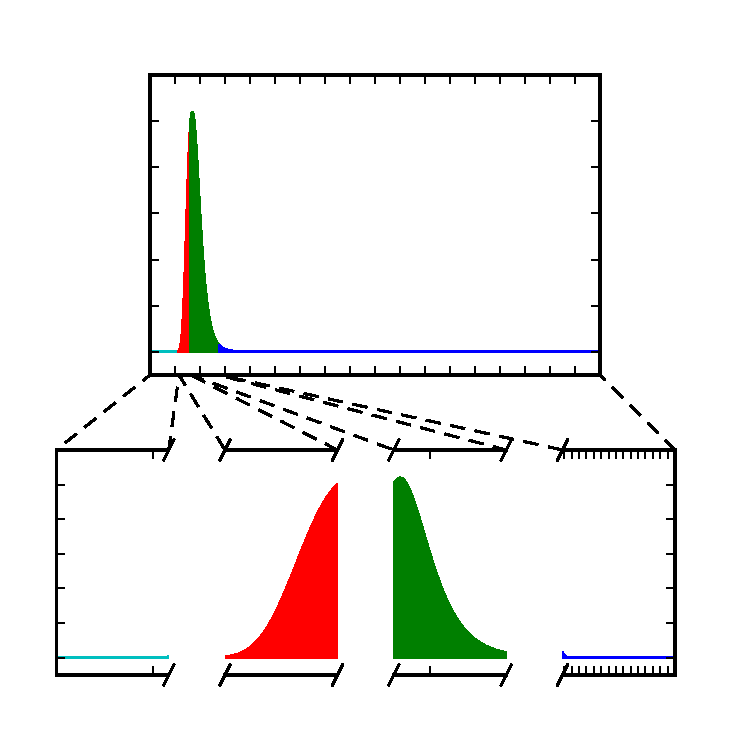
\includegraphics{radial_integrand}
    \end{center}
\end{figure}

The innermost integration is over $D_\mathrm{L}$ and is performed using adaptive Gaussian quadrature, but with a twist that speeds up convergence. As in many parameter estimation problems, the integrand may be sharply peaked, and any generic adaptive integration scheme may take a long time to find the peak. Before evaluating each inner integral over $D_\mathrm{L}$, the quantities $A=-\frac{1}{2} \sum_i {\rho_i}^2$ and $B=\sum_i \rho_i \hat\rho_i$ are precalculated so that the integrand can be written as
%
\begin{equation*}
	\exp\left(\frac{A}{{D_\mathrm{L}}^2} + \frac{B}{D_\mathrm{L}}\right) {D_\mathrm{L}}^m.
\end{equation*}
%
Then, we see that the likelihood $\exp(A {D_\mathrm{L}}^{-2} + B {D_\mathrm{L}}^{-1})$ is maximized when $D_\mathrm{L} = D_{\mathrm{L},0} = -2A/B$. The likelihood takes on a factor $\eta$ (say, $\eta=0.01$) of its maximum value when
%
\begin{equation}
	D_\mathrm{L} = D_{\mathrm{L},\pm} = \left(\frac{1}{D_{\mathrm{L},0}} \mp \sqrt{\frac{\log\eta}{A}}\right)^{-1}.
\end{equation}
%
We have now identified up to five breakpoints that partition the distance integrand into up to four intervals with quantitatively distinct behavior. These intervals are depicted in Figure~\ref{fig:radial_integrand} with distance increasing from left to right. There is a left\nobreakdashes-hand or small distance tail in which the integrand is small and monotically increasing, a left\nobreakdashes- and right\nobreakdashes-hand side of the maximum likelihood peak, and a right\nobreakdashes-hand tail in which the integrand is small and monotonically decreasing. These breakpoints are:
%
\begin{equation}
    D_{\mathrm{L},\mathrm{break}} = \{ D_\mathrm{L} \in
    \left\{
    \begin{array}{c}
    D_{\mathrm{L},\mathrm{min}} \\
    D_{\mathrm{L},-} \\
    D_{\mathrm{L},0} \\
    D_{\mathrm{L},+} \\
    D_{\mathrm{L},\mathrm{max}}
    \end{array}
    \right\} :
    D_{\mathrm{L},\mathrm{min}} \leq D_\mathrm{L}
    \leq D_{\mathrm{L},\mathrm{max}}\}.
\end{equation}
%
We use these breakpoints as initial subdivision in an adaptive Gaussian quadrature algorithm. Specifically, we use the GNU Scientific Library's \verb|gsl_integrate_qagp|\footnote{\url{http://www.gnu.org/software/gsl/manual/html_node/QAGP-adaptive-integration-with-known-singular-points.html}} function, which is designed to integrate functions with known singular points (though, of course, or integrand has no singular points). This function estimates the integral over each subdivision and each interval's contribution to the total error, then subdivides the interval whose error contribution is largest. Subdivisions continue until a fixed total fractional error is reached. In this way, most integrand evaluations are expended on the most important distance interval, whether that happens to be the tails (when the posterior is dominated by the prior) or the peak (when the posterior is dominated by the observations).


\ack Source code for \ac{BAYESTAR} is available on the \ac{LIGO} \acl{DASWG} web site at \url{http://www.lsc-group.phys.uwm.edu/daswg/projects/bayestar.html}.

Some of the results in this paper have been derived using \ac{HEALPix} \cite{healpix}.

\ac{LIGO} was constructed by the California Institute of Technology and Massachusetts Institute of Technology with funding from the \ac{NSF} and operates under cooperative agreement PHY\nobreakdashes-0107417. Some results were produced on the NEMO computing cluster operated by the Center for Gravitation and Cosmology at University of Wisconsin\nobreakdashes--Milwaukee under \ac{NSF} Grants PHY\nobreakdashes-0923409 and PHY\nobreakdashes-0600953. This research is supported by the \ac{NSF} through a Graduate Research Fellowship to L.S. This paper has \ac{LIGO} Document Number \ac{LIGO}\nobreakdashes-PXXXXXXX\nobreakdashes-vX.


\section*{References}
\bibliographystyle{iopart-num}
\bibliography{apj-jour,bib/telescope}

\end{document}
